% !TEX root = ..\thesis.tex


 







\chapter{ Mô hình}
% vẽ sơ đồ hệ thống

Mô hình tổng quan của đề tài hình \ref{fig:general_chart}
\begin{figure}[H]
    \centering
    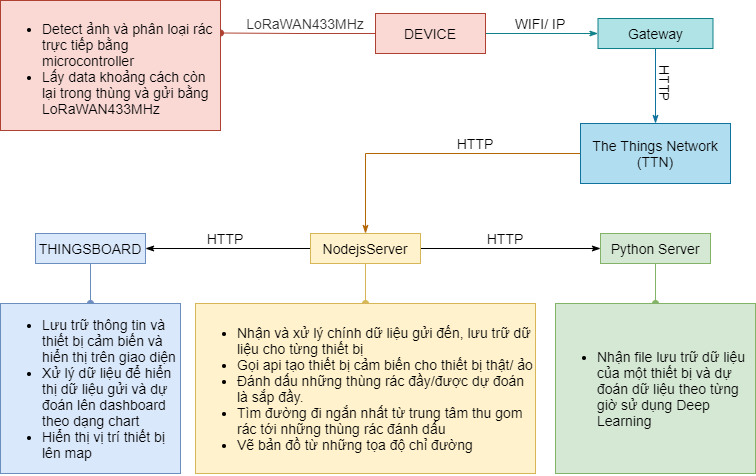
\includegraphics[width=\textwidth]{images/general_chart.png}
    \caption{Mô hình tổng quan}
    \label{fig:general_chart}
\end{figure}

Mô hình device \ref{fig:chart_smartbin}
\begin{figure}[H]
    \centering
    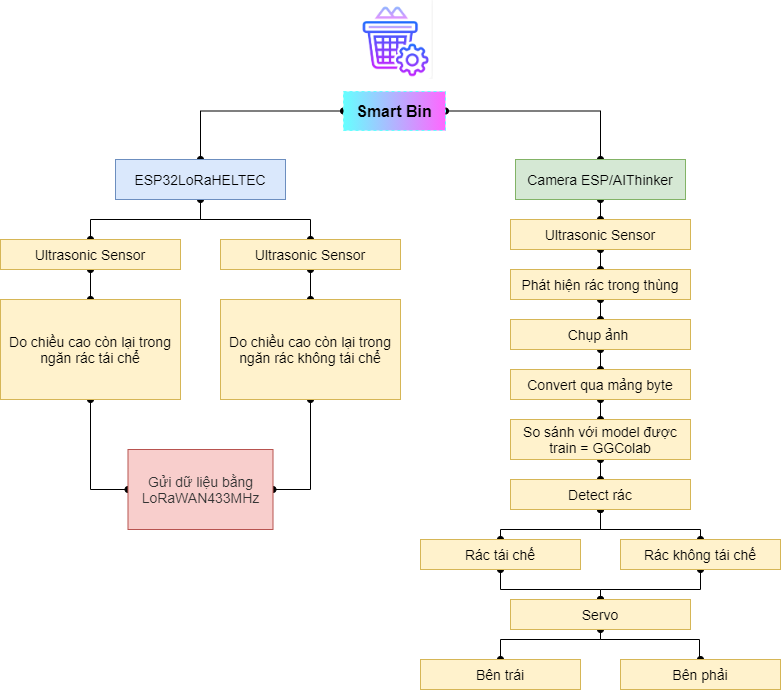
\includegraphics[width=\textwidth]{images/Chart_smartbin.png}
    \caption{Mô hình device}
    \label{fig:chart_smartbin}
\end{figure}

Mô hình server từ bước khởi tạo đến gửi dữ liệu \ref{fig:chart_server1}
\begin{figure}[H]
    \centering
    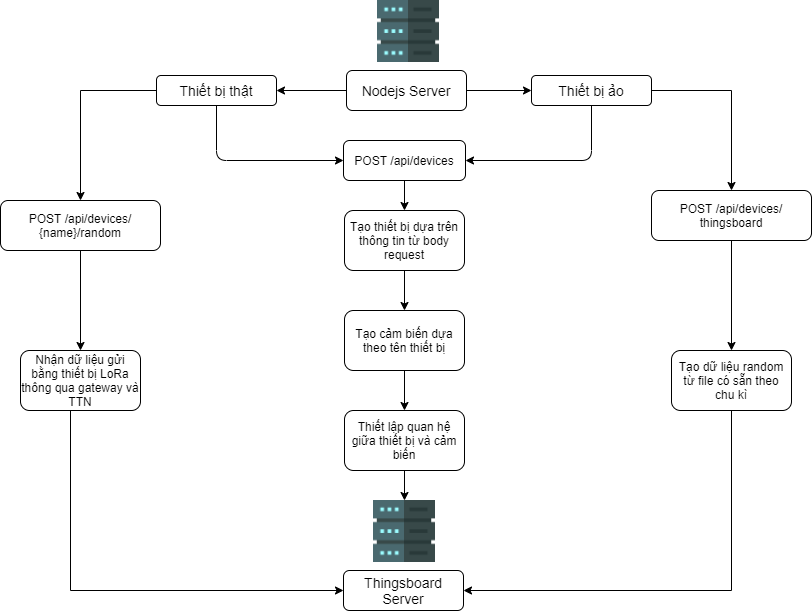
\includegraphics[width=\textwidth]{images/Khanh/Nodejs/Chart_server1.png}
    \caption{Mô hình server từ bước khởi tạo đến gửi dữ liệu}
    \label{fig:chart_server1}
\end{figure}

Mô hình server từ bước gửi dữ liệu đến xử lý bản đồ \ref{fig:chart_server2}
\begin{figure}[H]
    \centering
    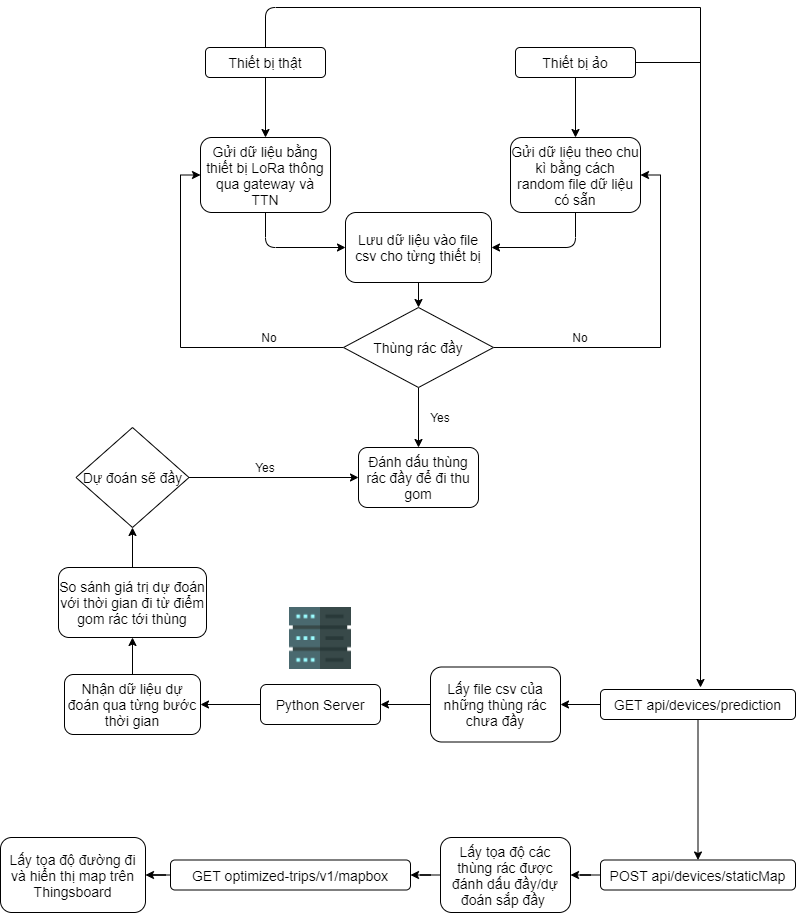
\includegraphics[width=\textwidth]{images/Khanh/Nodejs/Chart_server2.png}
    \caption{Mô hình server từ bước gửi dữ liệu đến xử lý bản đồ}
    \label{fig:chart_server2}
\end{figure}